
\documentclass{beamer}

%\usepackage{qtree}
\usepackage{beamerthemetree}
%\usepackage{beamerthemesplit}
\usepackage{color}
\usepackage{lingmacros}
\setbeamertemplate{footline}[frame number]
\usepackage{graphicx}
%\usepackage{xyling}
%\usepackage[swedish]{babel} 
\usepackage[latin1]{inputenc} 
\usepackage{natbib,avm}
\newcommand{\newblock}{}
\usepackage{hyperref}


\title{An Introduction to  Semantics using Type Theory with Records \\
  Lecture 4     }
\author{Jonathan Ginzburg\\
Universit\'e Paris-Diderot, Sorbonne Paris-Cit\'e\\
Robin Cooper\\ 
University of Gothenburg}
\date{}

\AtBeginSection[]
{
   \begin{frame}[plain]
       \frametitle{Outline}
       \tableofcontents[currentsection]
   \end{frame}
}

\newcommand{\backgroundyellow}{\beamertemplateshadingbackground{yellow!40}{magenta!20}}
\newcommand{\backgroundwhite}{\beamertemplateshadingbackground{white!100}{white!100}}
\newcommand{\ba}{\begin{avm}}
\newcommand{\ea}{\end{avm}}


\newenvironment{display}{\begin{center}}{\end{center}}

%
% Reference the next example in the text:
%
\newcommand{\nexteg}[1]{\addtocounter{examplectr}{1}(\arabic{examplectr}{#1})\addtocounter{examplectr}{-1}}
%
% Reference the previous example in the text:
%
\newcommand{\preveg}[1]{(\arabic{examplectr}{#1})}
%
% Reference examples by relative offsets:
%
\newcommand{\egnum}[2]{\addtocounter{examplectr}{#1}(\arabic{examplectr}{#2})\addtocounter{examplectr}{-#1}}
%
%
% ENVIRONMENTS
%
% Examples Environments
%
\newcounter{examplectr}
\newcounter{subexamplectr}[examplectr]
\renewcommand{\thesubexamplectr}{\alph{subexamplectr}}
%
% Sub-example Macro:
%
\newenvironment{subex}%
   {%\vspace*{-.8\baselineskip}
     \begin{list}
       {\alph{subexamplectr}.}%
       {\setlength{\topsep}{0in}
        \setlength{\leftmargin}{1em}%{0.25in}
        %\setlength{\listparindent}{-2em}
        %\setlength{\labelsep}{\baselineskip}
 \usecounter{subexamplectr} }
       }%
   {\end{list}}
%
% Single Example Macro
%
% \newenvironment{ex}%
%    { \refstepcounter{examplectr}
     
% \bigskip

%     % \begin{list}
%       % {
%        (\arabic{examplectr})%}%
%        % {%\setlength{\topsep}{0in}
% %         \setlength{\leftmargin}{4em}%{0.75in}
% %         \setlength{\labelsep}{\baselineskip}
% % }
%         \hspace*{1em}\begin{minipage}[t]{4in} 
% %\item
%    }%
%    {\end{minipage}

% \bigskip

%     %\end{list}
% }
% %
% % End of example macro
% %
\newcommand{\bit}{\begin{itemize}}
\newcommand{\eit}{\end{itemize}}
\newcommand{\ben}{\begin{enumerate}}
\newcommand{\een}{\end{enumerate}}
\newcommand{\ignore}[1]{}
\newcommand{\eeen}{\eenumsentence}
\newcommand{\subegref}[2]{(\ref{#1}\ref{#2})}

%\newcommand{\beg}{\begin{ex}}
%\newcommand{\eeg}{\end{ex}}
%\newcommand{\bseg}{\begin{subex}}
%\newcommand{\eseg}{\end{subex}}


\newcommand{\egstack}[1]{\begin{tabular}[t]{@{}l@{}} #1 \\ \\
  \end{tabular}}

%Records

\newcommand{\record}[1]{$\left[\mbox{\begin{tabular}{lcl} #1
\end{tabular}}\right]$} 
\newcommand{\smallrecord}[1]{$\left[\mbox{\begin{tabular}{@{}l@{}c@{}l@{}} #1
\end{tabular}}\right]$}

\newcommand{\field}[2]{#1 & = & #2}
\newcommand{\tfield}[2]{#1 & : & #2}
\newcommand{\smalltfield}[2]{#1:#2 & &}
\newcommand{\mfield}[3]{#1=#2 & : & #3}
\newcommand{\smallmfield}[3]{#1=#2:#3 & &}
\newcommand{\hfield}[2]{{\sc #1} & & #2}




\begin{document}
\maketitle


\ignore{
Lecture 4.
We provide a unified theory of metacommunicative and illocutionary interaction on the basis of the notion of Austinian locutionary propositions. This provides a basis for describing various linguistic phenomena occuring during grounding and clarification interaction.
}





\begin{frame}\frametitle{Grounding}


    
\bit


\item Grounding (Herb Clark and collaborators): A's dialogue move
  $m_{1}$ before it enters the common ground must be {\it grounded} by
  B. Grounding requires that {\it B understands $m_{1}$ relative to
    her own purposes.}
    
    
    \item Alwood:  `Contributions in the form of "acknowledging
feedback" are not needed to
constitute speech acts but rather to inform the interlocutor of the
extent to which his communicative objectives are met.'

\item Traum  1994: computationally explicit account; 
 fused into Conversational Discourse Representation Theory in
 collaboration with Massimo Poesio (PTT).

\item PTT
integrates grounding into the general semantic interpretation process, uses
DRT to account for anaphoric uses to previous utterances;
very detailed picture of the  common ground
subsequent to an utterance. 

\eit\end{frame}

\begin{frame}\frametitle{Failing to ground}

\bit
\item How to construe the grounding criterion?


\item Not so crucial to formalize {\it B understands $m_{1}$ relative to
    her own purposes.} if one concentrates on successful cases (for
  discussion of challenges to formalization see e.g.\ Traum 1999).


\item More crucial if one wishes to study {\it What are the
  consequences of grounding failure?}


%\item What is the proper characterization of the range and distribution of
%CRs?

%\item \textcolor[rgb]{0.98,0.00,0.00}{What does this tell us about the communicative process?}
\eit\end{frame}


\begin{frame}\frametitle{When grounding fails: {\it CRification}}

\eeen{
\item[] Tim:
          Could I have one of those (unclear)? 
 Dorothy:     Can you have what? 
 Tim:          Have one of those things. 
 Dorothy:           What things? 
 Tim:           Those pink things that af after we had our lunch. 
 Dorothy:           Pink things? 
 Tim:          Yeah.           Er those things in that bottle. 
 Dorothy:          Oh {\bf I know what you mean.}
          For your throat? 
}
\end{frame}


\begin{frame}\frametitle{When grounding fails: {\it CRification}}




\bit

\item Clarification Requests (CRs)---one of the most explicit pieces of
  evidence we have of the distribution of sources of {\it trouble} in
  interaction.

\item Occur approx 5\% of the time (BNC: `eh': 1943, pardon: 768)

\item More {\it difficult} cognitively: kids start producing only from
  approx.\ 30
  months; no evidence of non-human CRs.

\item Crucial tool of linguistic stability: evidence from simulations
  (see Macura and Ginzburg, 2008,
Macura 2007 PhD thesis)

\end{itemize}\end{frame}

\begin{frame}\frametitle{Purver et al taxonomy}

\bit

\item There are a wide range of forms of CRs that can follow a given
utterance---their characterization is an adequacy requirement for any
theory of dialogue context:

\item See Purver et al 2001, Purver, 2004, for the
  taxonomy of CRs used here.
  
\item  This is based on a random
sampling of the 10 million word dialogue subcorpus of the BNC
consisting of c.\ 150,000 words.  4\% of sentences were found to be
clarification requests.  

\eit\end{frame}

\begin{frame}\frametitle{CRs: form classification}


\eeen{\item A: Did Bo leave?
\item {\it Wot} B: Eh? / What? / Pardon?
\item {\it Explicit} B: What did you say? / Did you say `Bo' ?
\item {\it Literal reprise} B: Did BO leave? / Did Bo LEAVE?
\item {\it Wh-substituted Reprise} B: Did WHO leave? / Did Bo WHAT?
\item {\it Reprise sluice} B: Who? / What? 
\item {\it Reprise fragment} (CE) B: Bo? / Leave?
\item {\it  Gap} B: Did Bo \ldots ?
\item {\bf Filler}: A: Did Bo \ldots B: Win?
(Table I from Purver, 2006)
}

\end{frame}

\begin{frame}\frametitle{CRs: content classification}

\bit

\item Four classes of contents were identified: they can be exemplified in
the form of {\sf   Explicit}
CRs:

\eeen{
\item {\bf Repetition}: What did you say? Did you say `Bo'?
\item {\bf Clausal confirmation}: Are you asking if Bo left? You're
  asking if who left?
\item {\bf Intended Content}: What do you mean ()? Who is `Bo'? 
\item {\bf Correction}: Did you mean to say `Bro'?
}

\eit
\end{frame}

\begin{frame}\frametitle{CRs: content classification}

\bit

\item
 Many CR utterances are multiply ambiguous. The most extreme
case is RF, which seems able to exhibit all four readings, main two being clausal and intended-content:

{\footnotesize
\eeen{

\item Marsha:		yeah that's it, this, she's got three rottweilers now and\\
Sarah:		three? \\
Marsha:		yeah, one died so only got three now

\item[] Are you saying she's got THREE rottweilers now?
}}

{\footnotesize
\eeen{
\item[] Tim:
          Could I have one of those (unclear)? 
 Dorothy:     Can you have what? 
 Tim:          Have one of those things. 
 Dorothy:           What things? 
 Tim:           Those pink things that af after we had our lunch. 
 Dorothy:           Pink things? 
 Tim:          Yeah.           Er those things in that bottle. 
 Dorothy:          Oh {\bf I know what you mean.}
          For your throat? 

}}

\eit
\end{frame}

\ignore{
\begin{frame}\frametitle{CRs: content classification}

\bit

\item

The repetition reading is expressed most commonly by the {\sf wot}
lexical class when the target is the entire utterance:

\eeen{\label{fid1}
\item

Gary:		 when he's away (pause)
        things go, actually things go a lot smoother.\\
Clare:		Sorry?\\
Gary:		Things go a lot smoother when he's not here. (KSR)

\item s bust:		Great memorial I think really isn't it?\\
e bust:		Beg pardon?\\
s bust:		Be a good appropriate memorial if we can afford
it. (KM8)
}
\eit\end{frame}
}

\begin{frame}\frametitle{CR form and type as percentage of CRs -- demographic portion}


{\tiny
\hskip -5pt\begin{tabular}{|c||r|r|r|r|r|r|r|r|r||r|}\hline
 &{\tt expl}&{\tt lit}&{\tt sub}&{\tt slu}&{\tt rf}&{\tt gap}&{\tt fil}&{\tt wot}&{\tt oth}& 
Total\\\hline\hline

{\tt cla} & 4.1  &  4.7  &  1.0  &  11.3 &  24.8 &     0 &     0 &     0 &  0.5  &  46.5 \\\hline
{\tt int} & 6.2  &     0 &    0  &     0 &  1.8  &     0 &     0 &   5.7 &     0 &  13.6 \\\hline
{\tt rep} & 0.8  &     0 &  2.6  &  2.3  &  0.3  &  0.5  &  3.1  &  26.3 &     0 &  35.9 \\\hline
{\tt cor} & 1.0  &  0.5  &    0  &     0 &  1.0  &     0 &     0 &     0 &     0 &   2.6 \\\hline
{\tt oth} &    0 &     0 &    0  &     0 &  0.8  &     0 &     0 &  0.5  &     0 &   1.3 \\\hline
\hline
 Total    & 12.1 &  5.2  &  3.6  &  13.6 &  28.6 &  0.5  &  3.1  &  32.5 &  0.5  & 100.0 \\\hline
\end{tabular}
}

\end{frame}

\begin{frame}\frametitle{CR form and type as percentage of CRs -- demographic portion}
\bit

\item CRs were found to make up just under 4\% of sentences when calculated
over the demographic portion, or just under 3\% when calculated over
all domains.

\item Forms: Commonest: {\it wot} and
{\it reprise fragment} forms, with each making up over 25\% of
CRs. Explicit CRs and reprise sluices  also common, each
contributing over 10\% of CRs. Other forms are all around 5\% or less.

\item Readings: nearly 50\% of CRs--- clausal-conf
with the repetition (about 35\%) and int-content (about
15\%) non-trivial.
\eit\end{frame}

\begin{frame}\frametitle{CE: parallelism conditions}

\begin{itemize}

\item  The clausal-conf and intended-content readings 
involve distinct syntactic and phonological parallelism conditions.  

\item Clausal readings do not require phonological 
identity between target and source:

{\tiny
\eenumsentence{
\item A: Did Bo leave? B: My cousin? 

\item A: Did she annoy Bo? B: Sue? 
}}

\item syntactic parallelism: an XP used to
clarify an antecedent sub-utterance $u_1$ must match $u_1$
categorially:


{\tiny
\eenumsentence{\label{para-ex}
\item A: I phoned him. B: him? / {\#}he?
\item A: Did he phone you? B: he? / {\#}him?
\item A: Did he adore the book. B: adore? / {\#}adored? 
\item A: Were you cycling yesterday? B: Cycling?/biking?/{\#}biked?
}}

\end{itemize}\end{frame}


\begin{frame}\frametitle{CE: parallelism conditions}

\begin{itemize}

\item
Int-cont readings of CE do seem to involve (segmental) phonological
identity with their source.

\eenumsentence{
\item[(i)] A: Did Bo leave? B: Max? (cannot mean: int-cont reading: {\bf who are you referring 
to?})
 }

\end{itemize}\end{frame}



\begin{frame}\frametitle{Non-existent CRs}

\bit

\item Two of
the most highly researched areas in formal and computational grammar
are syntactic ambiguity (e.g. prepositional attachment) and scopal
ambiguity.

\item \textbf{not a single CR concerned with syntactic
  or scopal ambiguity has been found}, suggesting that either these are not
domains that involve much uncertainty for interlocuters in human
conversation, or that there is some factor that prevents their production.

\item See Ginzburg, 2012  for discussion of  constructed scope
  disambiguation CRs such as:

\eeen{\label{cr-scope11}\item[] 
\item[] A(1): The boys kept a cat. \\
B(2): A cat? One cat for all the boys or different ones?\\
A(3): They each kept a cat.
}

\end{itemize}\end{frame}


\begin{frame}\frametitle{Empirical Conclusions }
\bit
\item  Schegloff's claim: (applied to CRs, not self-repair) `Because anything in
talk can be a source of trouble, everything in conversation is, in
principle, ``repairable''.' 
use
\item Evidence from three corpus studies \cite{pgh01,rs04,riesermoore05} (two concern English
  conversations, one German; two involve task oriented conversations,
  the most comprehensive involves a wide range of primarily free
  unrestricted conversation types.)

\eit
\end{frame}
\begin{frame}\frametitle{Empirical Conclusions }
\bit
\item {\bf Restricted range of contents}: the function of CRs seems, to a
  very large extent, to consist of either (a)
  confirming or querying intended content or (b) requesting repetition of
  a misheard (sub)-utterance.
use
\item {\bf Syntactic and phonological parallelism}: CRs frequently exhibit
  (segmental) phonological parallelism with their source,  indeed for certain
form/content combinations this is a grammatical requirement; this requirement is
weakened to syntactic parallelisms for other constructions.

%\item {\bf Link between lexical category and clarificational
%  potential}: CRs about open class lexical items are easily understood
%  as querying their intended content, whereas CRs about closed class
%  lexical items are 

%\item Resolve early and deep: fragments, involving reused material,
%  are the overwhelming majority
 

\eit
\end{frame}


\begin{frame}\frametitle{  GRCR conditions   }

\bit
\item  The
  ability to characterize for any utterance type the update that
  emerges in the aftermath of successful mutual understanding ({\it grounding}), and  the
  full range of possible clarification requests (Clarification interaction  = CRification) otherwise.
\eit



\end{frame}

\frame[allowframebreaks]{\frametitle{What entity delivers GRCR conditions?
}

\bit

\item Need entity which (a) both CPs have interest in preserving,

\item from which range of CRs is derivable, 
\item and which
allows original speaker (Ariadne) to 
interpret and recognize the coherence of a class of possible
clarification queries that original addressee (Barabas) might make.

\item allows utterance presuppositions to be derived:

\eeen{\label{utt1} \item[]           

\noindent A(1): Did Mark send you a love letter?\\
B(2b): No, though it's interesting {\bf that you refer to Mark/my
brother/our friend}  \\     
B(2d): No, though it's interesting {\bf that you ask about Mark's epistolary
habits}\\ 
B(2e): No, though it's interesting {\bf that the final two words you 
just uttered start with `l'}
  }
\eit

}

\begin{frame}\frametitle{What entity delivers GRCR conditions?
}

\bit

\item Content: pro: in Ariadne's  DGB post-utterancely; con: not necessarily in Barabas'; too coarse grained.

\item Meanings (Montague/Kaplan sense): pro:  range of contextual parameters offers a possible
characterization of the contextually variable and hence potentially
problematic constituents of utterance content.

\item if we conceive of
meanings as entities which characterize potential sources of
misunderstanding, then at a minimum all open class words
 will also need to be assumed to project parameters
which requiring instantiation in context.
\eit

\end{frame}

\begin{frame}\frametitle{What entity delivers GRCR conditions?
}

\bit



\item Con 1: coarse grained

\eenumsentence{\label{grain-prob}
\item Ariadne: Jo is a lawyer. Barabas: A lawyer?/What do you 
mean a lawyer?/{\#}What do you mean an advocate?/{\#}What do you 
mean an attorney?
\item  Ariadne: Jo is an advocate. Barabas: {\#}What do you 
mean a lawyer?/An advocate?/What do you mean an advocate?/{\#}What do you 
mean an attorney?
}

Con 2: need syn/phon data to ensure potential for syntactic and
phonological parallelism (e.g. for CE).



\eit

\end{frame}

\begin{frame}\frametitle{Sub-utterance potential for CRs}

\bit
\item {\it a priori} ANY sub-utterance is
clarifiable (but significant caveats qualitatively and quantitatively):

%EXAMPLES

\eeen{\label{all-constits}
\item Who  rearranged the plug behind the table?

\item  Who? /  rearranged?/ the plug? / behind? / the table?

\item A: Is that the shark? B: The? B: Well OK, {\it A}. (based on an
  example in the film {\it Jaws}.)
}


\item The consequences this has for utterance representation is that we need
to ensure that for a given utterance each {\it sub}-utterance is
accessible as an antecedent.


\end{itemize}\end{frame}
\ignore{
\begin{frame}\frametitle{Keeping Track of Constituents}

\bit

 \item In HPSG phrasal constituency handled in terms of the feature
   {\sc dtrs}. 
\item {\sc dtrs} is limited to immediate constituents, but by
  recursion we eventually have access to more remote constituents. 
\item Concretely, a token of a sentential type will have values for
  all sub-utterances in paths emanating from the highest level {\sc
    dtr}. 


\item Two possible strategies: the first is to enable access to  non-immediate
constituents by expressive means that in some way effect a recursion, an approach implemented by \cite{lappin-gregory99}





\eit
\end{frame}

\begin{frame}\frametitle{Keeping Track of Constituents}

\bit
\item The other strategy, adopted here---enhance the representation
  itself so it  keeps track of {\it all} constituents not merely the
  immediate ones. 
\item This is done by positing an additional, set valued field in the type definition of signs dubbed {\sc constit(uent)s}




\eit
\end{frame}
}

\begin{frame}\frametitle{ An utterance type}

 \begin{avm}
\[
{\sc phon} : {\tt is georges here}\\
{\sc cat} = V[+fin] : syncat\\
constits =  \{is, georges, here, is georges here\} : set(sign)\\
{\sc c-params}   : \[
spkr: IND\\
addr: IND\\
c1 : address(s,a)\\
s0: SIT\\
l: LOC\\
g: IND\\
c3: Named(g,`georges')\]\\
cont = Ask(spkr,addr, ?\[sit = s0\\
sit-type = In(l,g)\]) : IllocProp
\]\end{avm}


\end{frame}


\begin{frame}\frametitle{What entity delivers GRCR conditions?
}

\bit 
\item The locutionary proposition defined by u, $T_u$ is a grammatical
  type that classifies $u$ is the proposition \begin{avm}\[sit = u\\
    sit-type = T$_u$\]\end{avm}.
This will deliver GRCR conditions.

\item Why the grammatical type: 
\begin{itemize}
\item Finer grain than content, meaning 
\item syn/phon parallelism with source utterance
\end{itemize}

\item Why the utterance token: 
\begin{itemize}
\item Need instantiated content, not merely meaning
\item Reference to sub-utterances tokens figure in CRs (`Bo?' = Who referring to
in that utterance of `Bo'.)
\end{itemize}
\end{itemize}

\end{frame}

\begin{frame}\frametitle{A locutionary proposition}

{\tiny
\eenumsentence{
\item[]

 \begin{avm}\[ sit = \[
phon = {\tt dijoliv}\\
cat = V[+fin,+root]\\
constits = \{di,jow,liv\}\\
dgb-params = \[
 s0 = sit0\\
t0 = time0\\
j = j0\\
c3 = c30\]\\
cont = ([])\[sit = s0\\
sit-type = Leave(j,t0)\] 
\]\\
sit-type =\[
{\sc phon} : {\tt did jo leave}\\
{\sc cat} = V[+fin,+root] : syncat\\
constits = \{did, jo, leave\} : set(sign)\\
{\sc dgb-params} : \[
s0: SIT\\
t0: TIME\\
j: IND\\
c3: Named(j,jo)\]\\
cont = ([])\[sit = s0\\
sit-type = Leave(j,t0)\] : Questn
\]\]\end{avm}
}
}
\end{frame}



\begin{frame}\frametitle{Incorporating metacommunicative interaction}

\begin{itemize}

\item Add resource: Pending---incompletely processed utterances.

\item In light of need for  fine grainedness and non-semantic parallelism:\\
Change type of resource
 Moves, Pending keep track of
$ \langle$ utt. token, utt. type $\rangle$ pair ({\it locutionary propositions})


\item New defn of DGBType:

\begin{avm}\[spkr: Ind\\
                             addr: Ind\\
                             utt-time: Time\\
                           c-utt : addressing(spkr,addr,utt-time)\\
                        Facts : Set(Prop)\\
                      {\bf  Pending :  list(LocProp)}\\
                           Moves : list(LocProp)\\
                           QUD : poset(Question)\]\end{avm}
      

\end{itemize}\end{frame}



\begin{frame}\frametitle{Incorporating metacommunicative interaction}

\begin{itemize}


\item Grounding: utterance type fully classifies utterance token

\item CRification: utterance type calculated is weak (e.g.\ incomplete
  word recognition); need further
  information to spell out token (e.g.\ incomplete contextual resolution).

\end{itemize}
\end{frame}




\begin{frame}\frametitle{Pending: composition }

\bit
\item Utterances are kept track of
  in a contextual attribute {\sc pending} in the immediate aftermath of the speech event.

\item Given a presupposition that $u$ is the most recent speech event
and that $T_u$ is a grammatical type that classifies $u$, a record of the form \begin{avm}\[sit = u\\ sit-type = T$_u$\]\end{avm} (of type LocProp ({\it locutionary proposition})), gets added to {\sc pending}.

\eit
\end{frame}


\begin{frame}\frametitle{Contextual extension}

\bit

\item Contextual instantiation will of
course occur as soon as an utterance has taken place, but it can also
take place subsequently, as when more information is provided as a
consequence of CRification

{\footnotesize \eeen{\item[]
{\bf  Contextual extension}

 given the MaxPending locutionary proposition p = \ba\[sit
=u\\sit-type =T$_u$\]\ea and a record $w$ that (a) contextually
extends $u$ and such that (b) $w.c-params$ is a subrecord of the
c-param anchoring intended by u's speaker, integrate $w$ into
$p$.
}}

\end{itemize}\end{frame}




\begin{frame}\frametitle{CRification}

\bit
\item
Failure to fully instantiate contextual parameters or recognize
phonological types triggers CRification. 


\item This involves 
 accommodation of questions into context by means of a particular
 class of conversational rules---Clarification Context
  Update Rules (CCURs). 

\item We can do this given the highly restricted nature of potential
  CRs, given our corpus results.
  
    \eit
  
  \end{frame}




\frame[allowframebreaks]{\frametitle{CRification}

\bit
  \item Each CCUR specifies
  an accommodated MaxQUD built up from  sub-utterance u1  of the target utterance {\it MaxPending}.
  
  
  \item 
 Common to all CCURs is a license to follow up {\it MaxPending} with an utterance which is
 {\it co-propositional} with MaxQud
 

\item We can define {\it CoPropositionality} as follows:

\bit
\item Two utterances $u_0$ and
  $u_1$ are {\it co-propositional} iff the questions $q_0$ and $q_1$
  they contribute to QUD are co-propositional.  

\item $q_0$ and $q_1$ are co-propositional if there exists a record $r$
  such that $q_0(r) = q_1(r)$. 

\eit

 \item In practice: {\it co-propositional} here: either a CR which differs
from MaxQud at most in terms of its domain, or a correction---a
proposition that instantiates MaxQud. 

\item Example: `Whether Bo left', `Who left', and `Which student left' (assuming Bo
  is a student.)

\eit
}



\begin{frame}\frametitle{CRification}

\bit
\item {\sf Parameter identification}: 
\ba\[pre :
\[Spkr : Ind\\
        MaxPending : LocProp\\
            u0 $\in$ MaxPending.sit.constits \]\\
effects: \[
          MaxQUD =   $\lambda x(Mean(pre.spkr,u0,x)$ : Question\\
      LatestMove : LocProp\\
          c1: CoProp(LatestMove.cont,MaxQUD)\]
          \]\end{avm}

\eit
\end{frame}


\begin{frame}\frametitle{Parameter Identification}

\begin{itemize}

\item Underpins CRs such as:

\eenumsentence{\item[] A: Is Bo here?
\item Who do you mean `Bo'?

\item WHO?

\item Bo? (= Who is `Bo'?)
}

\item Example shortly; NSU cases tomorrow.

\item We can also deal with corrections, as in (\ex{1}). B's corrective utterance is 
co-propositional with $\lambda x$Mean(A,u2,x), and hence allowed in by
the specification.

\eeen{\label{gr-ext121}
\item A: Is Bo here?
\item B: You mean Jo.
}

\end{itemize}
\end{frame}

%\ignore{

\begin{frame}\frametitle{Incorporating metacommunicative interaction}
\bit
%\item Simple example exemplifying the origin of the Turn Taking Puzzle
\item Single (public) input leads to distinct outputs on `public
  level'.
\eit
\end{frame}

\begin{frame}\frametitle{ The Turn Taking Puzzle}

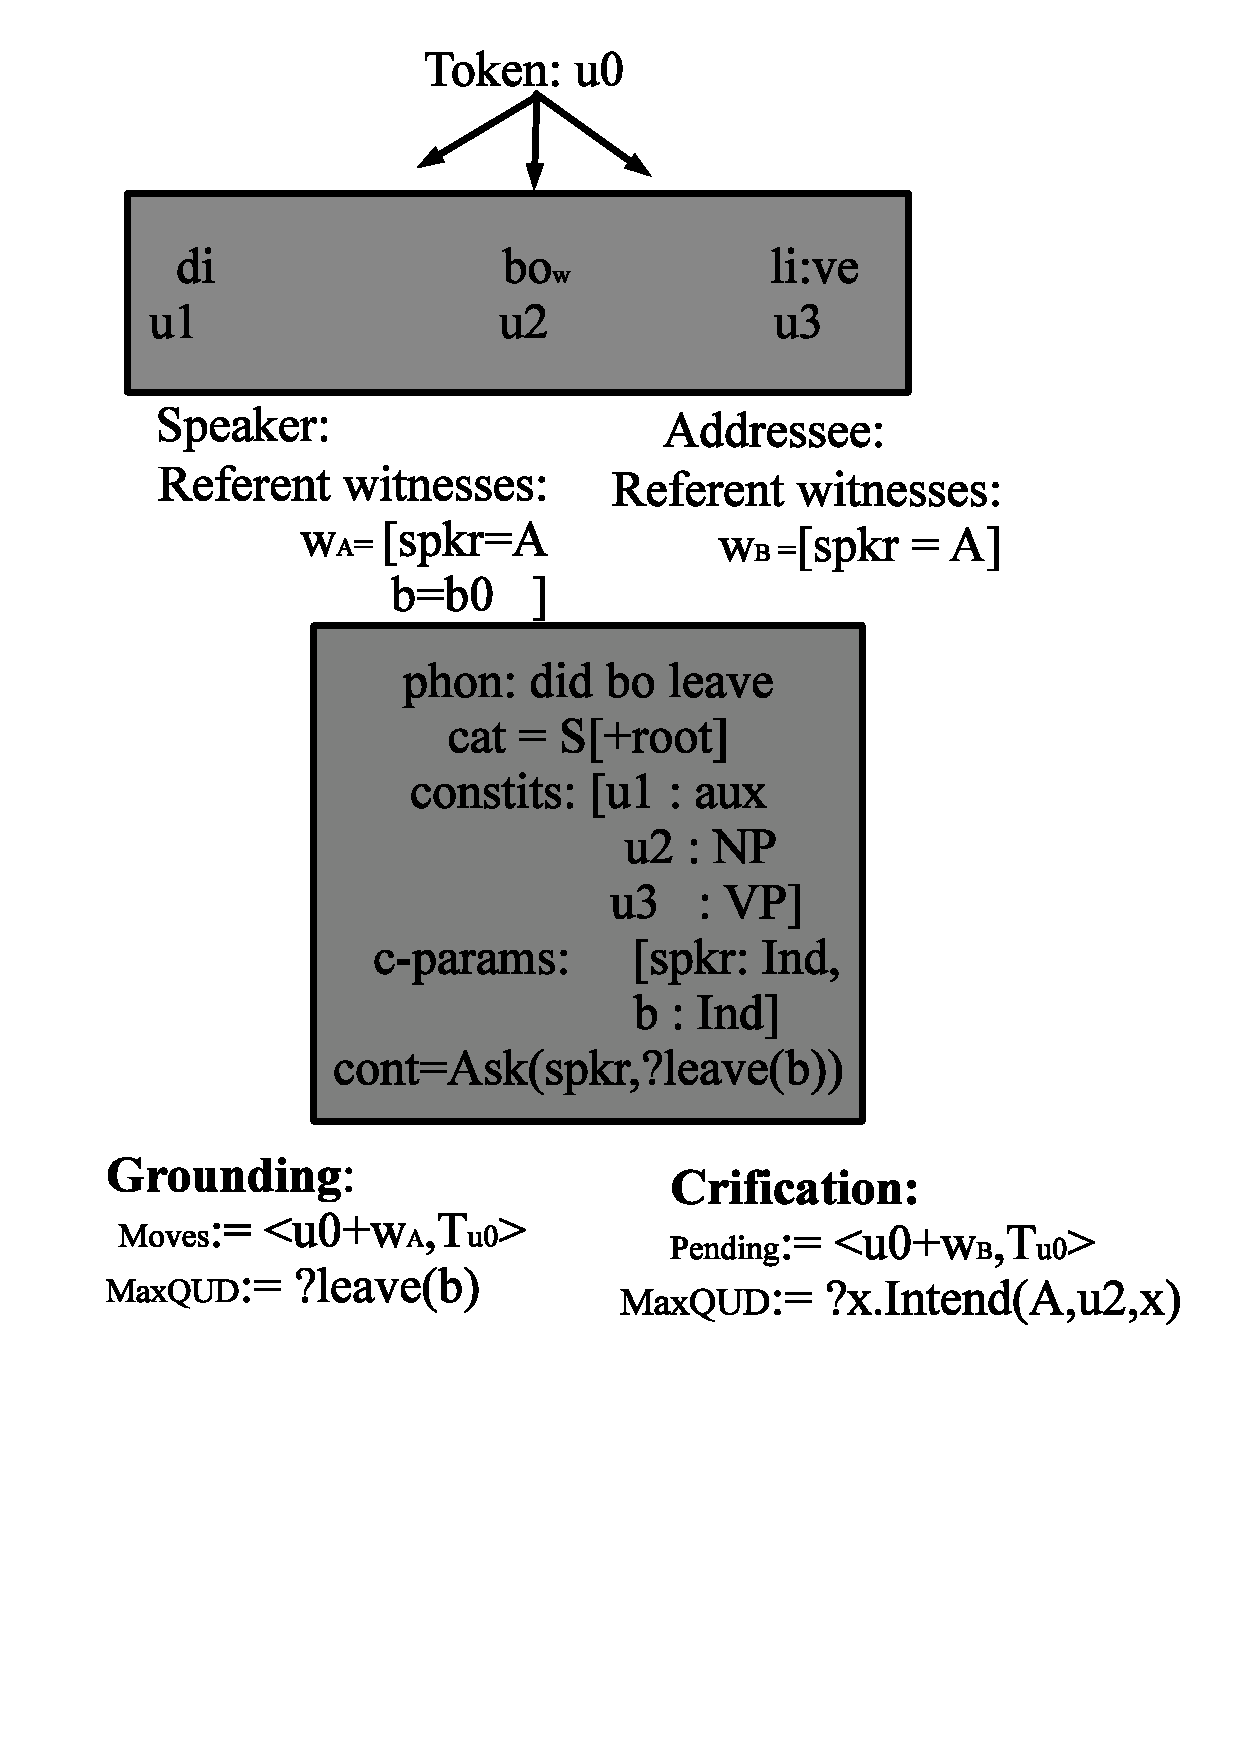
\includegraphics[height=8cm,width=8cm]{grounding-crex-rev.pdf}

\end{frame}

\begin{frame}\frametitle{An example}

\eeen{\item[] A(1): Is Georges here?\\ B(2):  WHO do you mean?\\
A(3): George Sand.\\ B:(4) Ah,(5) no.
}

\end{frame}


\begin{frame}\frametitle{Example}

{\scriptsize
\begin{avm}\[
T$_u$ =  IGH  \\
u = u0\\
dgb0 =                  \[spkr = A\\
                             addr = B\\
                             Pending = \< \>\\
                             Moves = \< \>\\
                                      qud = \<\ \>\\
                                      facts = \{ \ldots   In(l,\{A,B\}),\\
 MostRecentSpeechEvent(u0),\\
 Classify(IGH,u0), \ldots\}
\] 
\]
\end{avm}
}
\end{frame}

\begin{frame}\frametitle{Example}

{\scriptsize

 dgb2' = \ba
\[
spkr =  A\\
addr =  B \\
pending = \<\[sit = w0'\\
\[ phon = izjorjhiya\\
         cat = V[+fin,+root] \\
       constits = \{v1(iz),v2(jorj),\\v3(hiya),v4( izjorjhiya)\}\\
                             dgb-params = \[
                                                    spkr = A\\
                                                    addr = B\\
                                                    time = t0\\
                                                     s0 = sit1\\
                                                      l =l0\\
                                                      c3 =  pr1\]\\
                                                   cont = Ask(spkr,addr, ?\[sit = s0\\
                                                                 sit-type = In(l,g)\])\]\\
                       sit-type = IGH\]\>\\
qud = dgb0.qud\\
facts = dgb0'.facts\\
moves = \< \>\]\ea
}
\end{frame}

\begin{frame}\frametitle{Example}

{\scriptsize
\ba
\[
spkr =  B\\
addr =  A \\
T$_u$ = WDYM\\
u = u1\\
pending = \<\[sit = w0'\\
                       sit-type = IGH\]\>\\
c3 = pr3\\
q1 = $\lambda x$ Mean(pre.spkr,pre.v2,x)  : Questn\\
qud = \<q1 \>\\
facts = facts1' = dgb0.facts $\cup$  \{MostRecentSpeechEvent(u1)\}\\
moves = \<\[sit = w1\\
                       sit-type = WDYM\]\>
\]\ea
}
\end{frame}


\begin{frame}\frametitle{Example}

{\scriptsize
\ba
\[
spkr =  B\\
addr =  A \\
pending = \<\[sit = w0'\\
                       sit-type = IGH\]\>\\
qud = \< $\lambda x$Mean(A,v2,x)\>\\
facts = facts1'\\
moves = \<Ask(B,A,$\lambda x$Mean(A,v2,x))\>
\]\ea
}
\end{frame}





\begin{frame}\frametitle{An example}

{\scriptsize
\eeen{\label{pivot}
%\item[] A: Is Georges here? B: Is WHO here?
\item
A.dgb7 = \ba
\[
spkr =  B\\
addr =  A \\
pending = \<\[sit = w1\\
                    sit-type = WDYM\] \>\\
qud = \<p1?\>\\
facts = \{   In(l,\{A,B\}) \\
         Named(`Georges',g),\\
2ndMostRecentSpeechEvent(u0),  \\ Classify(IGH,u0)     \\
MostRecentSpeechEvent(u1),  \\ Classify(WDYM,u1)     \}\\
moves = \<\[sit = w0\\
                       sit-type = IGH\]\>
\]\ea
}}

\end{frame}

\begin{frame}\frametitle{An example}
{\scriptsize
\eeen{
\item[] B.dgb7' = 
\ba
\[
spkr =  B\\
addr = A\\
pending = \<\[sit = w0'  \\
                       sit-type = IGH\]\>\\
qud = \<$\lambda x$Ask(A,B,?In(l,x))\>\\
facts = \{  In(l,\{A,B\}) \\
         Named(`Georges',g),\\
2ndMostRecentSpeechEvent(u0),  \\ Classify(IGH,u0)     \\
MostRecentSpeechEvent(u1),  \\ Classify(WDYM,u1)     \}\\
moves = \<\[sit = w1\\
                    sit-type = WDYM\]\>
\]\ea
}}

\end{frame}




\begin{frame}\frametitle{The TTP revisited}

\bit

\item  A has the question of {\it whether Georges is here} as the sole
member of {\sc qud}, whereas the utterance `WHO do you mean?' remains
pending;


\item remains pending because  no applicable LatestMoveUR.

\eit
\end{frame}
\begin{frame}\frametitle{The TTP revisited}

\bit


\item In
contrast, B's QUD consists of the question {\it who do you mean}, whereas the utterance `Is Georges here' is
pending.

\end{itemize}\end{frame}
\begin{frame}\frametitle{The TTP revisited}
\bit
\item  However, TTP-type mismatches are exhibited intrinsically on the level of
production, but need not arise at the level of comprehension.  

\item That
is, in the current example---and more generally---it is rarely the
case that the author of an utterance $u$ fails to understand CRs
relating to $u$, let alone to recognize their coherence.

\eeen{\item[] A: Who does Bo admire? b: Bo?}


\item In order to enable this possibility, we offer a rule that {\it inter
  alia} allows the integration of CRs concerning $u$ by the author of
$u$.

\end{itemize}\end{frame}


\begin{frame}\frametitle{CR Accommodation}

\bit
\item CCUR.qud(u1)---question accommodated by applying a CCUR to u1.


\item {\it CR accom rule}: if the speaker of
LatestMove is the current addressee, $p$ is pending, and u1 is a
constituent of LatestMove, one can update moves with $p$ and QUD with
CCUR.qud(u1), so long as $p$ is co-propositional with CCUR.qud(u1).
\eit
\end{frame}



\begin{frame}\frametitle{An example}
{\scriptsize
A.dgb8 = \ba
\[
spkr =  B\\
addr =  A \\
pending = \< \>\\
qud = \< $\lambda x$Ask(A,B, ),  p1?\>\\
facts = dgb7.facts\\
moves = \<\[sit = w1\\
                    sit-type = WDYM\] ,\\\[sit = w0\\
                       sit-type = IGH\]\>
\]\ea
}
\end{frame}



\begin{frame}\frametitle{An example}

\eeen{
\item A(3): (I'm asking about) George Sand. B:(4) Ah,(5) no.
}
\end{frame}



\begin{frame}\frametitle{An example}
{\scriptsize
B.dgb8' = 
\ba
\[
spkr =  A\\
addr = B\\
pending = \<\[sit = w0'  \\
                       sit-type = IGH\]\>\\
qud = \<?Mean(A,v2,gs)<,$\lambda x$Ask(A,B,$\lambda x$Mean(A,v2,x))\>\\
facts = dgb7'.facts\\
moves = \<\[sit = w3\\
sit-type = GS\],\\
\[sit = w1\\
                    sit-type = IWH\]\>
\]\ea
}
\end{frame}



\begin{frame}\frametitle{An example}
{\scriptsize
B.dgb9' = 
\ba
\[
spkr =  B\\
addr = A\\
pending = \<\[sit = w0'  \\
                       sit-type = IGH\]\>\\
qud = \< \>\\
facts = \{Ask(A,B,Mean(A,v2,gs))\}\\
$\cup$ dgb7'.facts\\
moves = \<\[sit = w4\\
sit-type = Ah\],\\\[sit = w3\\
sit-type = GS\],\\
\[sit = w1\\
                    sit-type = IWH\]\>
\]\ea
}
\end{frame}



\begin{frame}\frametitle{An example}
{\scriptsize
B.dgb10' = 

\ba
\[
spkr =  B\\
addr = A\\
pending = \< \[sit = w0 = \[  dgb-params = \[
                                                    spkr = A\\
                                                    addr = B\\
                                                    time = t0\\
                                                     s0 = sit1\\
                                                      l =l0\\
                                                      g = gs\\
                                                      c3 =  pr1\]\\
                                                      cont = Ask(spkr,addr, ?\[sit = s0\\
                                                                 sit-type = In(l,g)\])\]\\
                       sit-type = IGH\]\>\\
qud = dgb9'.qud\\
facts = dgb9'.facts\\
moves = dgb9'.moves
\]\ea
}
\end{frame}



\begin{frame}\frametitle{An example}
{\scriptsize

 B.dgb11' = 
\ba
\[
spkr =  B\\
addr = A\\
pending = \< \>\\
qud = dgb9'.qud\\
facts = dgb9'.facts\\
moves = \<\[sit = w0\\
sit-type = IGH\], dgb10'.moves \>\\
\]\ea
}
\end{frame}



\begin{frame}\frametitle{An example}
{\scriptsize

B.dgb12' = 
\ba
\[
spkr =  B\\
addr = A\\
pending = \< \>\\
qud = \< ?In(lo,gs)\>\\
facts = dgb9'.facts\\
moves = dgb11'.moves
\]\ea
}\end{frame}




\begin{frame}\frametitle{Summary}

%\includegraphics{flow2.eps}
%\begin{figure*}[!h]
%\begin{center}
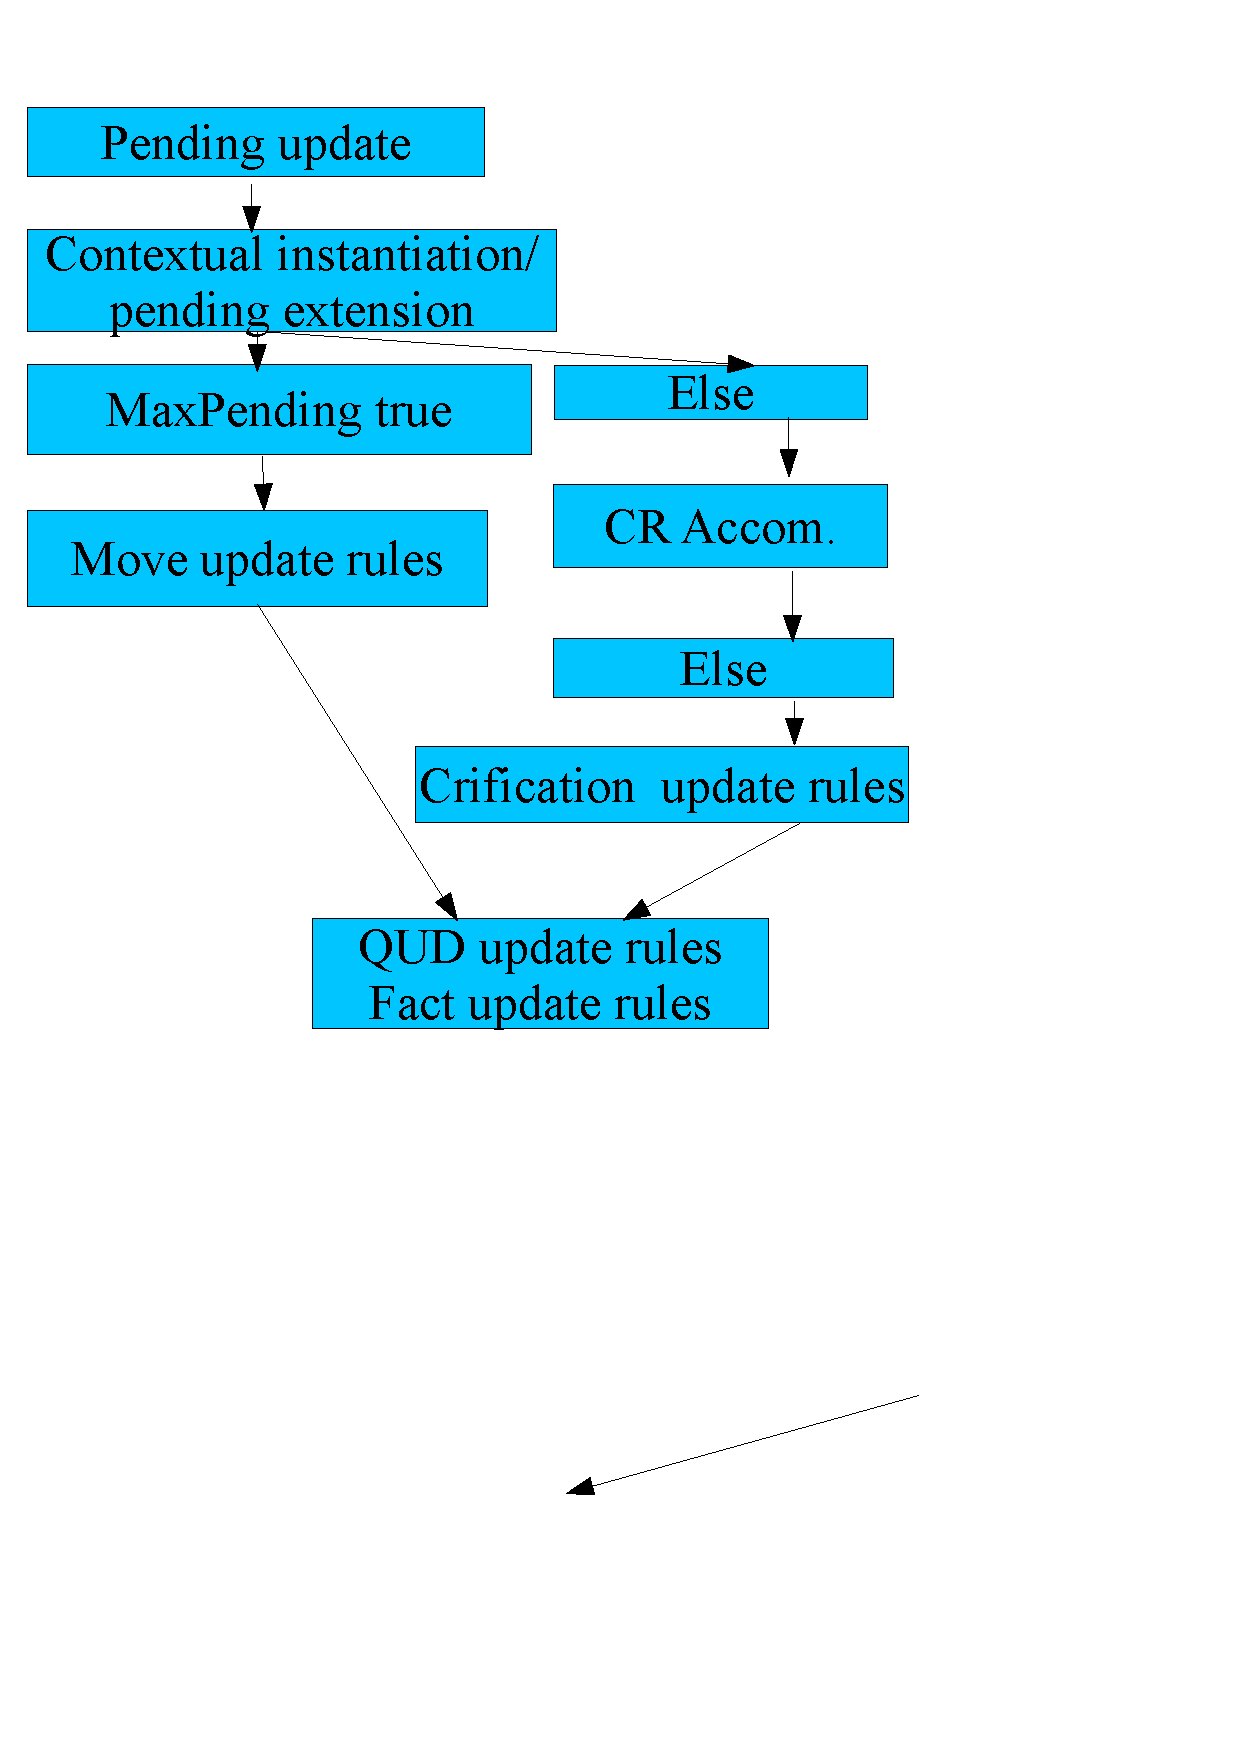
\includegraphics[height=9cm,width=8cm]{flow2.pdf}
%\caption{Sketch of Interrogatives type hierarchy from Ginzburg and Sag 2000} \label{int-hi}
%\end{center}
%\end{figure*}

\end{frame}



\bibliographystyle{natbib}
\bibliography{newest-jg-fin}

\end{document}

\ignore{



}

